% !TEX encoding = UTF-8 Unicode

\documentclass[twocolumn,10pt,a4j]{ltjsarticle}
\usepackage{kougai}

\title{ゲームに最適化されたベンチマークソフト「FlexBench」開発}
\author{2032087 大司 陽輝  指導教員 須田 宇宙 准教授}
\date{}

\begin{document}

\maketitle

\section{はじめに}
近年では,CPUやGPUの発展に伴いゲームの需要が増加し、その中でも、よりグラフィカルな表現力があり、MODを使用することでクリエイティブな楽しみ方ができるゲーミングPCが注目される。しかし、ゲーミングPCを購入するには専門的な知識を要する。
そこで、ベンチマークソフトを使うことでパソコンの客観的な性能を図ることができるが、ゲームによって要求されるスペックが異なるため参考にしにく、初心者にはわかりにくい点がある。
そこで、本研究では、従来のベンチマークソフトよりゲームに忠実性を持たせつつ、パーツごとにゲームに対して評価を行うことで初心者にもわかりやすいようにしたベンチマークソフトの開発を行う。

\section{ゲームについて}
ゲームのグラフィックスは,近年進化を遂げている.従来のゲームでは,解像度はHD(1920$\times$1080ピクセル)程度であり,光の反射や陰影は簡易的なアルゴリズムによって表現されていた.しかし,最新のゲームでは,解像度は4K(3840$\times$2160ピクセル)や8K(7680$\times$4320ピクセル)といった高解像度になる。
光の反射はレイトレーシングという技術により,より実際の映像に近いものとなっている.レイトレーシングとは,光の光線が物体に当たったときにどのように反射や屈折するかを計算する技術で,ゲームのリアリティを大幅に向上させることができる.

\section{ベンチマークについて}
ベンチマークとは、特定の環境下においてパソコンの持つ性能をスコア化したものであり、CPUやGPUなどの性能を客観的に計測する指標を知ることができる。
ベンチマークは、自分のパソコンの性能を確認する時や、パソコンの購入の参考として使用することがある。
しかし、現状のベンチマークソフトでは、初心者に対してわかりにくい点と、ゲームに対して再現性が低いという二つの問題点がある。

 \subsection{ベンチマークソフト、初心者に対してわかりにくい点}
ベンチマークソフトは、性能を客観的に計測し性能をわかりやすくするためのものであるが、現状のベンチマークソフトの結果は数値で評価されることが多く、初心者にはどれくらいの性能かを判断するには難しい。また、全体性能を数値で評価された結果、性能をアップデートするにあたって、どの性能が不足しているかなどを判断するのもむずかしい。

 \subsection{ゲームに対して再現性が低い}
ゲームは、同様の挙動でも実装方法によって、CPU/GPUに対しての負荷のかかわり方が異なる。
そのため、現状のベンチマークソフトを実行し、高い評価を得られたとしても、実際プレイしたいゲームで快適に動作できるとは限らない。

\section{開発を行うベンチマークソフトについて}
そこで、本研究では、ベンチマークソフトの結果をPCの全体性能を数値として評価するのではなく、パーツごとの使用率から評価を行うことで、初心者でもわかりやすいように実装し、解像度や、レイトレーシング、シェーダーを変更できるようにすることで、より汎用性の高いベンチマークソフトの開発を行う。
シェーダーとは対象物の表面の描画における陰影処理を行うプログラムのことを指し、

\section{実装}
まず、現状のゲームがどういった要因で処理に時間がかかっているかを調べた。
結果としては、解像度やレイトレーシング(予測:検証します)、陰影をよりリアルに描写するための技術、フィールド内の草をリアルに表現する技術などが処理に時間がかかり、パフォーマンスが落ちていた。
そこで本研究では、解像度の変更と、レイトレーシングの設定を変更できるような機能を追加する。

\section{開発したベンチマークソフトからわかったこと}



\begin{figure}[h]
\begin{center}
 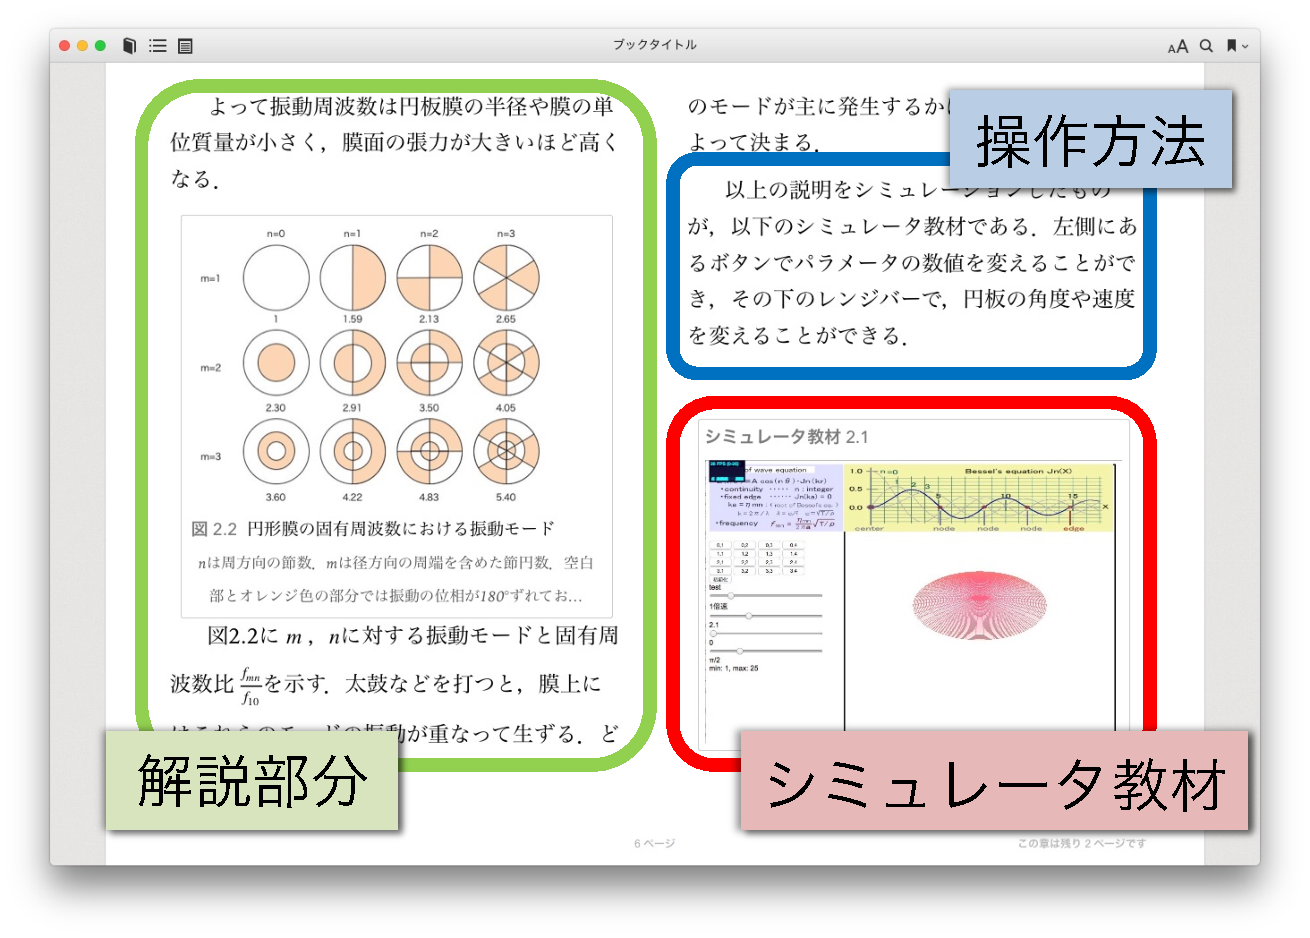
\includegraphics[clip,width=85mm,height=55mm]{textbook.pdf}
\end{center}
 \caption{電子教科書サンプル}
 \label{fig:教科書}
\end{figure}

\section{やること・やったこと}

論文や書籍から,ゲームで行われるグラフィックなどの処理を学び,開発を行うベンチマークソフトの参考とする.


\section{今後の予定}
Unityで,ゲームと同様の処理を行えるソフトの開発を行う

\begin{thebibliography}{99}
\bibitem{1} 須田宇宙: ``音響科学e-Learning教材'', \url{https://www.youtube.com/watch?v=rZdvL0ju4CA&ab_channel=TheSpyHood}, 2018/7/19参照
\end{thebibliography}

\end{document}
